%%% File encoding is ISO-8859-1 (also known as Latin-1)
%%% You can use special characters just like �,� and �


\chapter{Telling a History: Setting the inductive Scenario} 

in this chapter we will develop the story that will lead us to understand UGC11680. First, we explain the historical context and the study of physical processes extragalactic objects. Second, we exemplify our peculiar galaxy and try to see that part of this "history" fits into the overall framework. This will allow us to tell a story, step by step, without being redundant in the subsequent analysis.




\section{Tracers of star formation}
Star formation is an important facet of galaxy evolution caught "in the act". Much of the history of a galaxy is written through changes in its stellar population, inextricably linked through the processes of starbirth and stellar evolution. We can ask whether the current level of star formation is comparable with its past level, or has increased or decreased markedly. There are several disparate tracers from various wavelength regimes which give insight to the rate of star formation averaged over different timescales. In fact, the optical and near-infrared regimes are distinguished by being the only parts of the electromagnetic spectrum in which we can easily see any but the youngest stars in galaxies.

The first tracer of star formation to be developed and extensively used involves optical emission lines. The recombination lines from hydrogen have a particularly straightforward relationship to the number of ionizing photons from the hottest stars, which yields a star-formation rate (SFR) when coupled with stellar models and an initial-mass function.

In equilibrium, the number of photoionizations over the whole volume of gas
ionized by a star will equal the number of recombinations as the liberated electrons become bound to protons again. This generally happens only after many weaker Coulomb encounters, which have the helpful effect of making the velocity distribution of the electrons thermal (Maxwellian) even though it would have been quite different immediately upon their ejection from neutral atoms. During recombination, most electrons will be initially captured into an excited (high-n) state, and decay to the ground level by a cascade of photon emissions. The number of recombinations can thus be measured starting with the intensity of some emission line. This is usually one of the optical hydrogen lines (H, H), although instrumental advances have started to allow signifficant surveys using the infrared lines from transitions between higher pairs of n-values. These lines are intrinsically weaker in both energy and photon ux,
but have the enormous advantage of being much less sensitive to dust extinction.
Using the notation in Osterbrock and Ferland's treatment, a balance between
recombination and ionization requires that the number N LC of ionizing photons per second satisfy


where y is the frequency at the Lyman limit of hydrogen and  is the recombination coefficient, calculated including effects of resonent scattering which can keep essentially all atoms in n  2 in extensive nebul\ae. For comparison with observations, we use the calculations of what fraction of decay cascades leads to a given emission line, which may either be derived from a full cascade matrix incorporating all processes between the various levels, or using emissivities so derived for various lines at the relevant electron temperature. An effective recombination  eff rate can be defined,
such that the emission rate of photons in the relevant emission line is simply n p n eeff .(For example, at a typical electron temperature 10 4 K, each H photon stands in for 8.5 recombinations, while an H photon results on average from nearly half of all recombinations.) The line luminosity will be this quantity, integrated over the nebular volume, as diminished by distance (via 4D 2 for small enough distances to be
Euclidean):

A set of young stars will give o a number N LC of photons below the Lyman limit, and if the surrounding gas has sufcient column density, all these will be absorbed and eventually lead to recombinations (the ionization-bounded case). If we have a model of the stars' spectra in this region (which is unobservable because of this very absorption), we can calculate the number of ionizing phtons per second (also known as Q) as

in which the spectrum is converted to photons from the more usual energy units.
A widely-used relation was derived by Kennicutt (1998), using models for the
ionizing continuum of hot stars. Extrapolating to the entire mass in stars with a Salpeter (1955) initial mass function of power-law form, it is:

in solar masses per year, while counting only those stars with masses above 10 solarmasses, which actually ionize surrounding hydrogen, it becomes:



\section{Population Sinthesis}

The light of normal galaxies originates from stars. Stellar
evolution is largely understood, and the spectral radiation of
stars can be calculated from the theory of stellar atmospheres.
If the distribution of the number density of stars is known
as a function of their mass, chemical composition, and
evolutionary stage, we can compute the light emitted by
them. The theory of population synthesis aims at interpreting
the spectrum of galaxies as a superposition of stellar spectra.
We have to take into account the fact that the distribution
of stars changes over time; e.g., massive stars leave the
main sequence after several 10 6 yr, the number of luminous
blue stars thus decreases, which means that the spectral
distribution of the population also changes in time. The
spectral energy distribution of a galaxy thus reflects its his-
tory of star formation and stellar evolution. For this reason,
simulating different star formation histories and comparing
them with observed galaxy spectra provides important clues
for understanding the evolution of galaxies. In this section,
we will discuss some aspects of the theory of population
synthesis; this subject is of tremendous importance for our
understanding of galaxy spectra.

The processes of star formation are not understood in detail;
for instance, it is currently impossible to compute the mass
spectrum of a group of stars that jointly formed in a molec-
ular cloud. Obviously, high-mass and low-mass stars are
born together and form young (open) star clusters. The mass spectra of these stars are determined empirically from
observations.
The initial mass function (IMF) is defined as the initial
mass distribution at the time of birth of the stars, such that
m/ dm specifies the fraction of stars in the mass interval of
width dm around m, where the distribution is normalized,


The integration limits are not well defined. Typically, one
uses m L  0:1M  because stars less massive than 
008M  do not ignite their hydrogen (and are thus brown
dwarfs), and m U 100M  , because considerably more
massive stars are not observed. Whereas such very massive
stars would in any case be difficult to observe because of
their very short lifetime, the theory of stellar structure tells
us that more massive stars can probably not form a stable
configuration due to excessive radiation pressure. The shape
of the IMF is also subject to uncertainties; in most cases, the
Salpeter-IMF is used,


as obtained from investigating the stellar mass spectrum
in young star clusters. It is by no means clear whether
a universal IMF exists, or whether it depends on specific
conditions like metallicity, the mass of the galaxy, cosmic
epoch, or other parameters. Given the difficulties of deter-
mining the shape of the IMF, apparent variations of the
IMF with epoch or environment may be attributed to other
effect, such as the specifics of the star-formation history in
galaxies. Therefore, there seems to be no clear direct indica-
tion that the IMF varies with environment. However, as will
be discussed in Chap. 10, some properties of high-redshift
galaxies are very difficult to understand if their IMF would
be the same as in our neighborhood. It has therefore been
suggested that the IMF in starbursts is different from that of
quiescent star formation such as we are experiencing in the
Milky Way.
The Salpeter-IMF seems to be a good description for stars
with M  1M  , whereas the IMF for less massive stars
is flatter. Note that, due to the steep slope of the IMF, most
of the stellar mass is contained in low-mass stars. However,
since the luminosity of main-sequence stars depends strongly
on mass, approximately as L / M 3 , most of the luminosity
comes from high-mass stars (see Problem 3.2).
The star-formation rate is the gas mass that is converted
into stars per unit time,

The metallicity Z of the ISM defines the metallicity of
the newborn stars, and the stellar properties in turn depend
on Z. During stellar evolution, metal-enriched matter is
ejected into the ISM by stellar winds, planetary nebulae,
and SNe, so that Z.t/ is an increasing function of time.
This chemical enrichment must be taken into account in
population synthesis studies in a self-consistent form.
Let S ;Z .t 0 / be the emitted energy per wavelength and
time interval, normalized to an initial total mass of 1M  ,
emitted by a group of stars of initial metallicity Z and age
t 0 . The function S;Z.t t 0 / .t 0 /, which describes this emission
at any point t in time, accounts for the different evolution-
ary tracks of the stars in the Hertzsprung?Russell diagram
(HRD)?see Appendix B.2. It also accounts for their initial
metallicity (i.e., at time t  t 0 ), where the latter follows
from the chemical evolution of the ISM of the corresponding
galaxy. Then the total spectral luminosity of this galaxy at a
time t is given by


thus by the convolution of the star formation rate with
the spectral energy distribution of the stellar population. In
particular, F.t/ depends on the star formation history. In order to compute S;Z.t t 0 / .t 0 /, models for stellar evolution and stellar atmospheresneeded. As a reminder

Fig. 3.32a displays the evolutionary tracks in the HRD. Each
track shows the position of a star with specified mass in the
HRD and is parametrized by the time since its formation.
Positions of equal time in the HRD are called isochrones
and are shown in Fig. 3.32b. As time proceeds, fewer and
fewer massive stars exist because they quickly leave the main
sequence and end up as supernovae or white dwarfs. The
number density of stars along the isochrones depends on the
IMF. The spectrum S ;Z.t t 0 / .t 0 / is then the sum over all
spectra of the stars on an isochrone?see Fig. 3.33b.
In the beginning, the spectrum and luminosity of a stellar
population are dominated by the most massive stars, which
emit intense UV radiation. But after  10 7 yr, the flux below
1000 � is diminished significantly, and after  10 8 yr, it
hardly exists any more. At the same time, the flux in the
NIR increases because the massive stars evolve into red
supergiants.
For 10 8 yr . t 10 9 yr, the emission in the NIR remains
high, whereas short-wavelength radiation is more and more
diminished. After  10 9 yr, red giant stars (RGB stars)
account for most of the NIR production. After 3  10 9 yr,
the UV radiation increases again slightly, due to blue stars on
the horizontal branch into which stars evolve after the AGB
phase, and due to white dwarfs which are hot when they are
born. Between an age of 4 and 13 billion years, the spectrum
of a stellar population evolves fairly little.
Of particular importance is the spectral break located at
about 4000 a which becomes visible in the spectrum after
a few 10 7 yr. This break is caused by a strongly changing
opacity of stellar atmospheres at this wavelength, mainly
due to strong transitions of singly ionized calcium and the Balmer lines of hydrogen. This 4000 a-break is one of the
most important spectral properties of the continuum stellar
emission in galaxies; as we will discuss in Sect. 9.1.2, it
allows us to estimate the redshifts of early-type galaxies from
their photometric properties?so-called photometric redshift
estimates.

\section{Color Evolution}
Detailed spectra of galaxies are often not available. Instead
we have photometric images in different broadband filters,
since the observing time required for spectroscopy is sub-
stantially larger than for photometry. In addition, modern
wide-field cameras can obtain photometric data of numer-
ous galaxies simultaneously. From the theory of popula-
tion synthesis we can derive photometric magnitudes by
multiplying model spectra with the filter functions, i.e., the
transmission curves of the color filters used in observations,
and then integrating over wavelength (A.25). Hence the
spectral evolution implies a color evolution, as is illustrated
in Fig. 3.34a.
For a young stellar population the color evolution is rapid
and the population becomes redder, again because the hot
blue stars have a higher mass and thus evolve quickly in
the HRD. For the same reason, the evolution is faster in
B  V than in V  K. It should be mentioned that this
color evolution is also observed in star clusters of different
ages. The mass-to-light ratio M=L also increases with time
because M remains constant while L decreases.
As shown in Fig. 3.34b, the blue light of a stellar popula-
tion is always dominated by main sequence stars, although
at later stages a noticeable contribution also comes from horizontal branch stars. The NIR radiation is first dominated
by stars burning helium in their center (this class includes
the supergiant phase of massive stars), later by AGB stars,
and after  10 9 yr by red giants. Main sequence stars never
contribute more than 20 \% of the light in the K-band. The
fact that M=L K varies only little with time implies that
the NIR luminosity is a good indicator for the total stellar
mass: the NIR mass-to-light ratio is much less dependent
on the age of the stellar population than that for bluer
filters.

\section{star Formation History and galaxy colors}

Up to now, we have considered the evolution of a stellar
population of a common age (called an instantaneous burst
of star formation). However, star formation in a galaxy takes
place over a finite period of time. We expect that the star
formation rate decreases over time because more and more
matter is bound in stars and thus no longer available to form
new stars. Since the star formation history of a galaxy is
a priori unknown, it needs to be parametrized in a suitable
manner. A ?standard model? of an exponentially decreasing
star formation rate was established for this,

where is the characteristic duration and t f the onset of
star formation. The last factor in (3.38) is the Heaviside step
function, Hx D1 for x  0, H.x/ D 0 for x < 0. This
Heaviside step function accounts for the fact that .t/ D 0
for t < t f . We may hope that this simple model describes the basic aspects of a stellar population. Results of this model are
plotted in Fig. 3.35a in a color-color diagram.
From the diagram we find that the colors of the population
depend strongly on  Specifically, galaxies do not become
very red if  is large because their star formation rate, and
thus the fraction of massive blue stars, does not decrease
sufficiently. The colors of Sb spirals, for example, are not
compatible with a constant star formation rate?except if the
total light of spirals is strongly reddened by dust absorption
(but there are good reasons why this is not the case). To
explain the colors of early-type galaxies we need  . 4 
10 9 yr. In general, one deduces from these models that a
substantial evolution to redder colors occurs for t . Since
the luminosity of a stellar population in the blue spectral
range decreases quickly with the age of the population,
whereas increasing age affects the red luminosity much less,
we conclude

The spectral distribution of galaxies is mainly deter-
mined by the ratio of the star formation rate
today to the mean star formation rate in the past,
today= h i.

One of the achievements of this standard model is that
it explains the colors of present day galaxies, which have
an age  10 billion years. However, this model is not
unambiguous because other star formation histories .t/
can be constructed with which the colors of galaxies can be
modeled as well.



\begin{figure}[H]
\centering
	\includegraphics[width=0.5\textwidth, angle =270]%
	{03_GraphicFiles/20_TimeUGC11680NED01_proc_elines.jpg}%
\caption[A cow]{Spatially resolved Star formation history (SFH) for the stellar surface density. each map represent a time slice and run from 
upper-right corner, reads from right to left and ends  the bottom-left corner. Also, Each map color represents the stellar mass assembly 
for each slice, following the colormap. Notice that each map is not cummulative}
\label{fig:1}
\end{figure}






\begin{figure}[H]
\centering
	\includegraphics[width=0.9\textwidth]%
	{03_GraphicFiles/figure_1.jpg}%
\caption[A cow]{Final Historiogram for UGC11680NED01}
\label{fig:1}
\end{figure}

\begin{figure}[H]
\centering
	\includegraphics[width=1\textwidth]%
	{03_GraphicFiles/figure_13.jpg}%
\caption[A cow]{Color-Mass Diagram for the CALIFA survey historiograms. Each bin is the average historiogram for each group. }
\label{fig:13}
\end{figure}





\begin{figure}[!ht]
\centering
% -------------- SUBFIGURE -1 -------------- %
\begin{subfigure}{
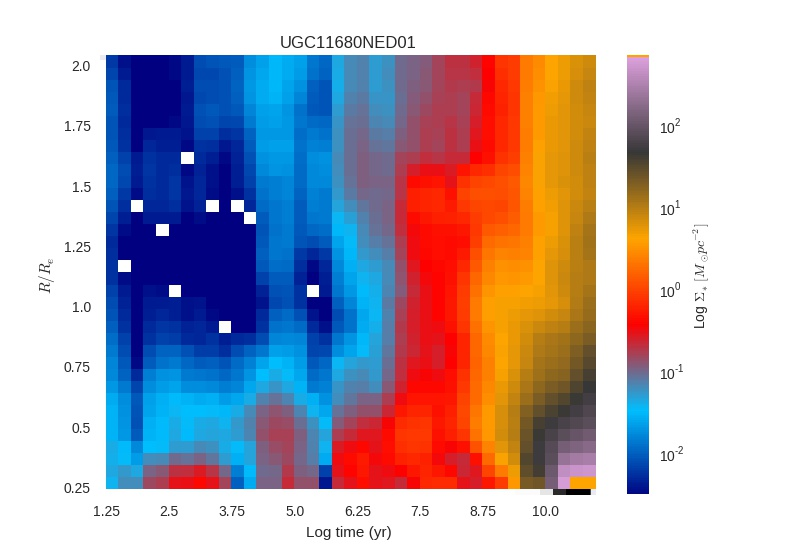
\includegraphics[width=.45\linewidth] {03_GraphicFiles/figure_1.jpg}   
\label{fig:subfig1} }
\end{subfigure}
\hfill
% -------------- SUBFIGURE -2 -------------- %
\begin{subfigure}{
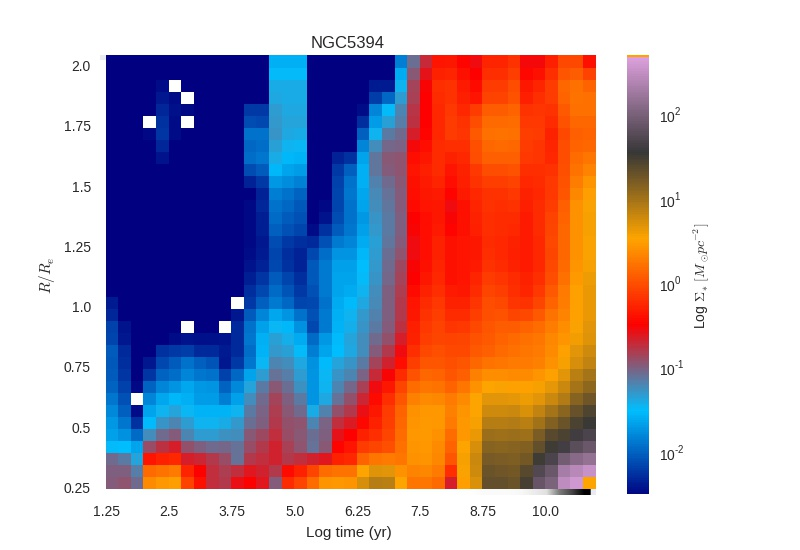
\includegraphics[width=.45\linewidth] {03_GraphicFiles/figure_2.jpg}
\label{fig:subfig2} }%
\end{subfigure}
\hfill
% -------------- SUBFIGURE -3 -------------- %
\begin{subfigure}{
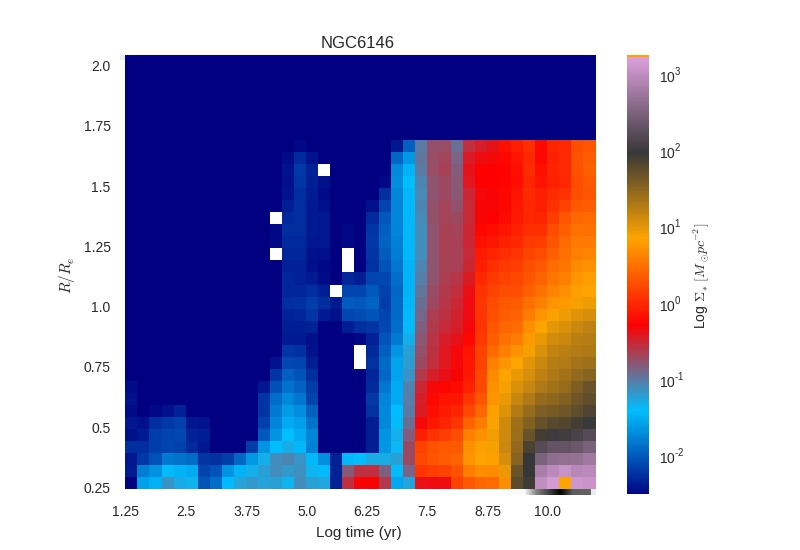
\includegraphics[width=.45\linewidth] {03_GraphicFiles/figure_3.jpg}
\label{fig:subfig3} }%
\end{subfigure}%
\hfill
% --------------SUBFIGURE -4 -------------- %
\begin{subfigure}{
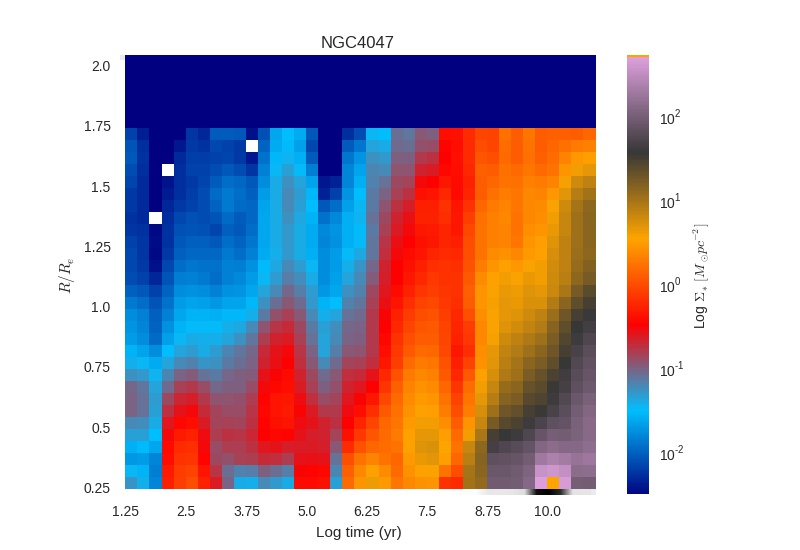
\includegraphics[width=.45\linewidth] {03_GraphicFiles/figure_4.jpg}
\label{fig:subfig4} }%
\end{subfigure}%
 
\label{myfigure}                            % label to the whole figure
\caption{Four Historiograms for different galaxies:UGC11680NED01,the red spiral. NGC5394,a interacting starburst galaxy.NGC6146,a typical elliptical 
galaxy and NGC4047,a face-on blue spiral.}
\end{figure}



\chapter{Dude (looks like an AGN)}


\begin{figure}[H]
\centering
	\includegraphics[width=1\textwidth]%
	{03_GraphicFiles/figure_14.png}%
\caption[A cow]{Color-Mass Diagram for the CALIFA survey. Each bin includes the mass assembly history tracks for different effective radius (nucleus,
middle range and outskirts) The time scale is linear. Notice the inside-out grow in stellar mass. }
\label{fig:14}
\end{figure}


\begin{figure}[H]
\centering
	\includegraphics[width=1\textwidth]%
	{03_GraphicFiles/figure_15.jpg}%
\caption[A cow]{Color-Mass Diagram for the CALIFA survey. Each bin includes the mass assembly history tracks for different effective radius (nucleus,
middle range and outskirts) The time scale is logarithmic. Notice the inside-out grow in stellar mass. }
\label{fig:15}
\end{figure}




\chapter{The $\chi^2$ Measure}

For a > 0, the gamma function G(a) is defined by


The most important properties of the gamma function are the following:

A continuous random variable X is said to have a gamma distribution if the
pdf of X is

Figure 4.26(a) illustrates the graphs of the gamma pdf for several (a, b) pairs, whereas
Figure 4.26(b) presents graphs of the standard gamma pdf. For the standard pdf,
when a 1, f(x; a) is strictly decreasing as x increases; when a > 1, f(x; a) rises to a maximum and then decreases. The parameter b in (4.7) is called the scale parameter
because values other than 1 either stretch or compress the pdf in the x direction.


DEFINITION Let n be a positive integer. Then a random variable X is said to have a chi squared distribution with parameter n if the pdf of X is the gamma density with a 1?4 n/2 and b 1?4 2. The pdf of a chi-squared rv is thus

The chi-squared distribution is important because it is the basis for a number
of procedures in statistical inference. The reason for this is that chi-squared
distributions are intimately related to normal distributions




\begin{figure}[!ht]
\centering
% -------------- SUBFIGURE -1 -------------- %
\begin{subfigure}{
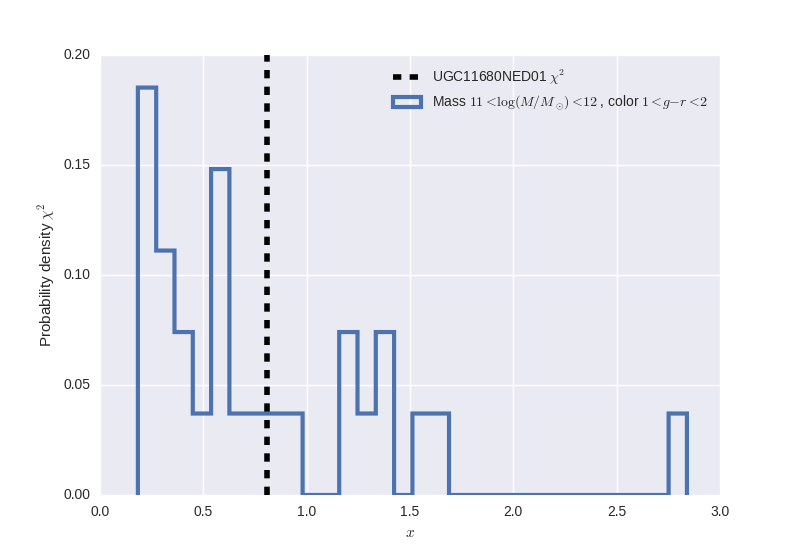
\includegraphics[width=.45\linewidth] {03_GraphicFiles/figure_27.png}   
\label{fig:subfig27} }
\end{subfigure}
\hfill
% -------------- SUBFIGURE -2 -------------- %
\begin{subfigure}{
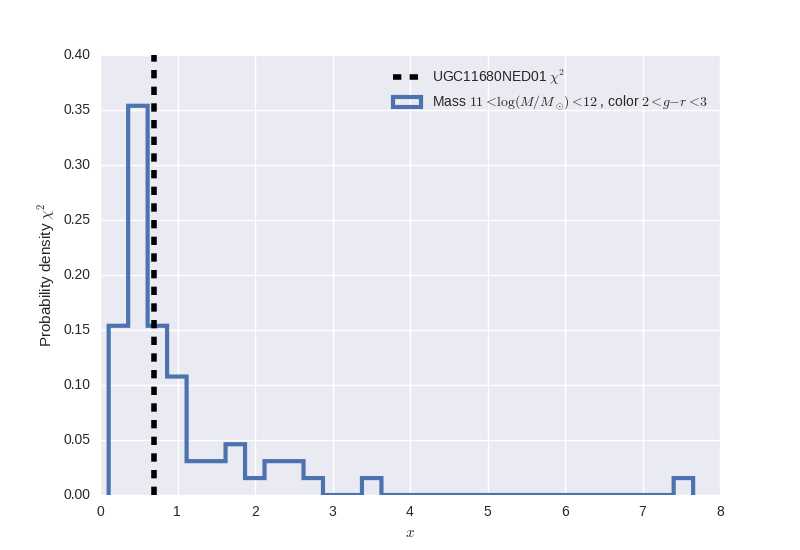
\includegraphics[width=.45\linewidth] {03_GraphicFiles/figure_26.png}
\label{fig:subfig28} }%
\end{subfigure}
\hfill
% -------------- SUBFIGURE -3 -------------- %
\begin{subfigure}{
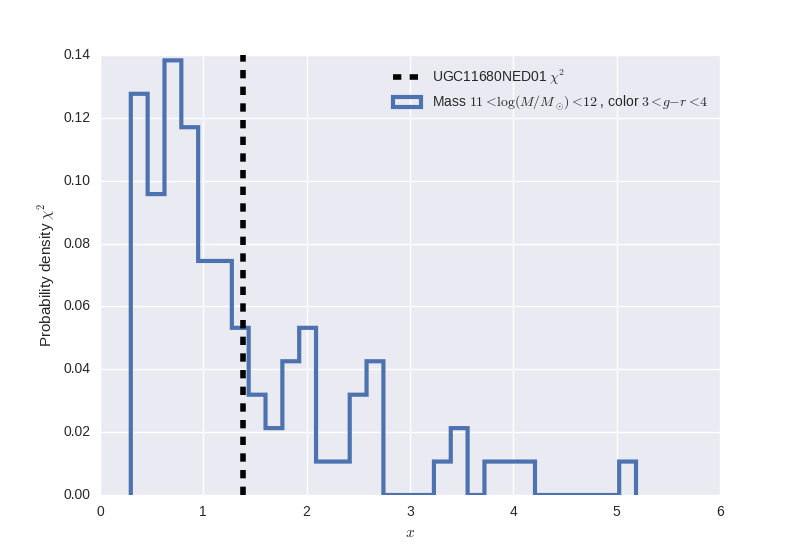
\includegraphics[width=.45\linewidth] {03_GraphicFiles/figure_24.png}
\label{fig:subfig29} }%
\end{subfigure}%
\hfill
% --------------SUBFIGURE -4 -------------- %
\begin{subfigure}{
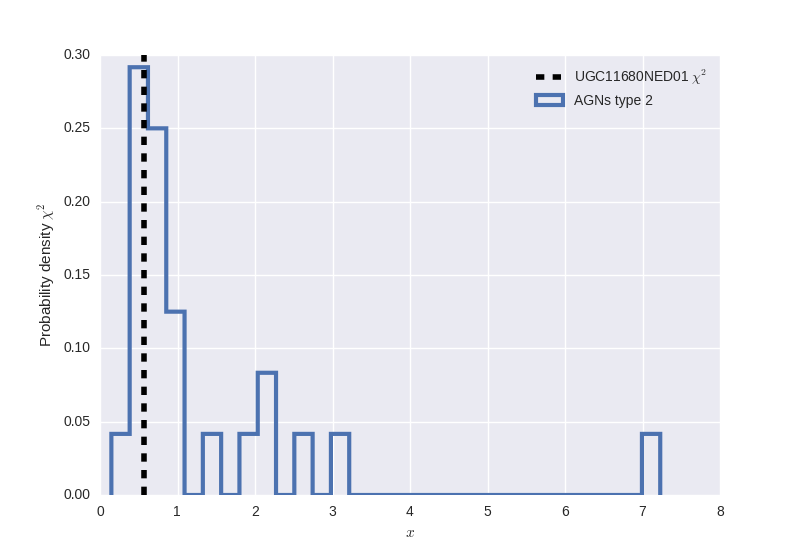
\includegraphics[width=.45\linewidth] {03_GraphicFiles/figure_32.png}
\label{fig:subfig30} }%
\end{subfigure}%


 
\label{myfigure}                            % label to the whole figure
\caption{$\chi^2$ reducided distribution for all galaxies in the mass range $11<\log (M/M_{\odot})<12$  in the CALIFA survey, subdivided by color $g-r$ bins. The Black dashed line represents
the $\chi^2$ reducided value of UGC11680NED01 compared with each mass bin average. The bootom-right figure is the all AGNS $\chi^2$ reducided distribution}
\end{figure}





\begin{figure}[!ht]
\centering
% -------------- SUBFIGURE -1 -------------- %
\begin{subfigure}{
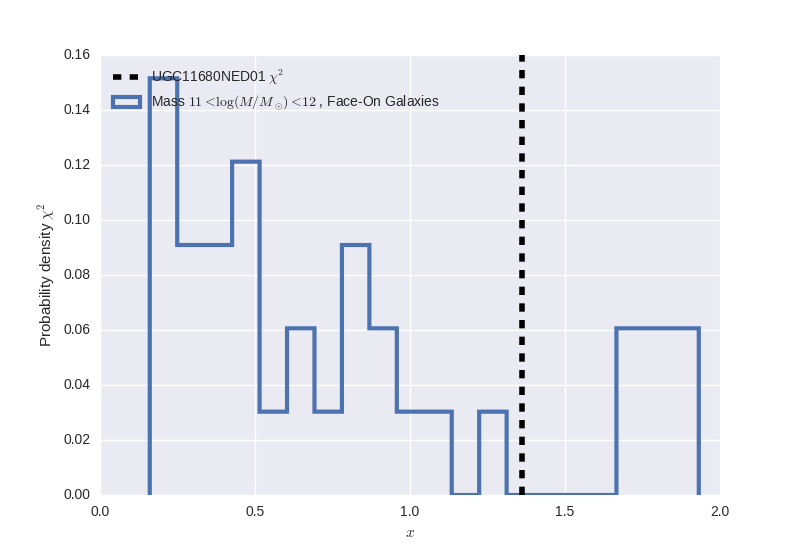
\includegraphics[width=.45\linewidth] {03_GraphicFiles/figure_34.png}   
\label{fig:subfig34} }
\end{subfigure}
\hfill
% -------------- SUBFIGURE -2 -------------- %
\begin{subfigure}{
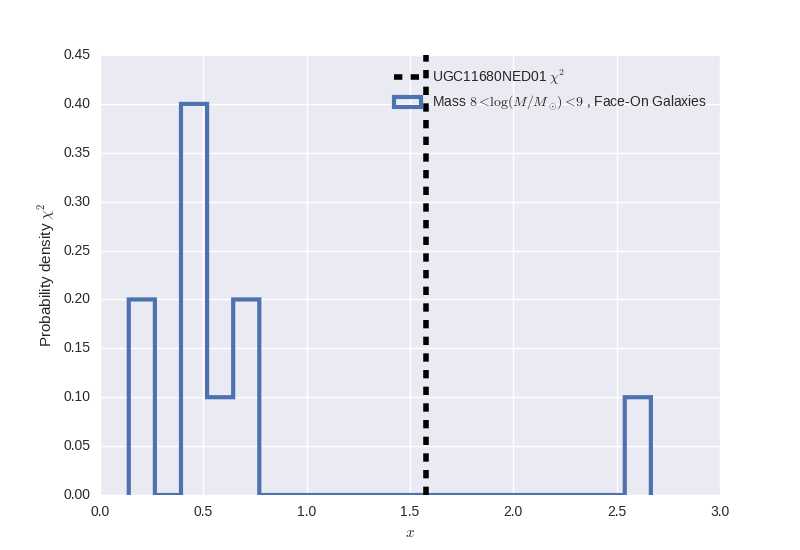
\includegraphics[width=.45\linewidth] {03_GraphicFiles/figure_35.png}
\label{fig:subfig35} }%
\end{subfigure}
\hfill
% -------------- SUBFIGURE -3 -------------- %
\begin{subfigure}{
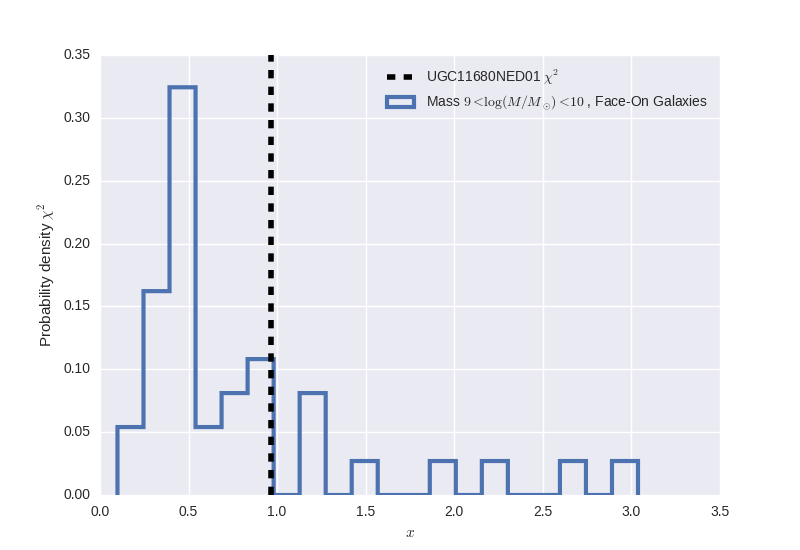
\includegraphics[width=.45\linewidth] {03_GraphicFiles/figure_37.png}
\label{fig:subfig37} }%
\end{subfigure}%
\hfill
% --------------SUBFIGURE -4 -------------- %
\begin{subfigure}{
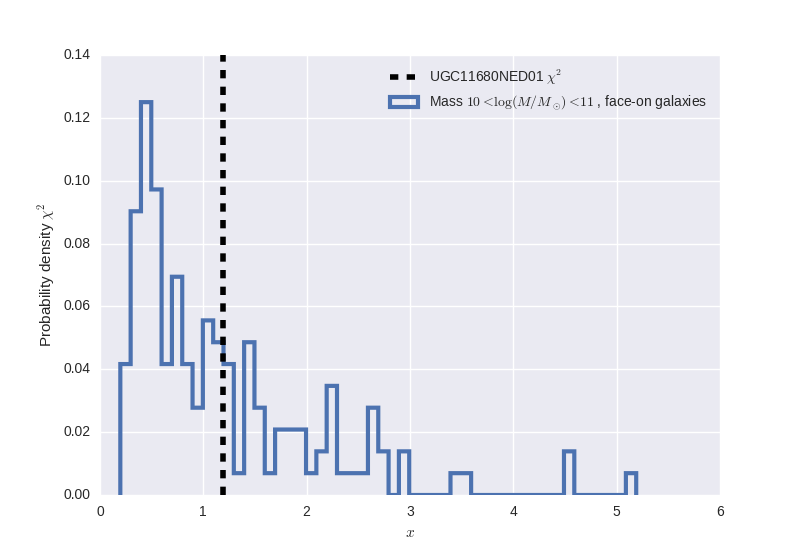
\includegraphics[width=.45\linewidth] {03_GraphicFiles/figure_38.png}
\label{fig:subfig38} }%
\end{subfigure}%
 
\label{myfigure}                            % label to the whole figure
\caption{$\chi^2$ reducided distribution for all Face-On Spiral Galaxies in the CALIFA survey, subdivided in mass bins. The Black dashed line represents
the $\chi^2$ reducided value of UGC11680NED01 compared with each mass bin average}
\end{figure}



